\documentclass{article}
\usepackage[utf8]{inputenc}
\usepackage{listings}
\usepackage[french]{babel}
\usepackage{graphicx}
\usepackage[left=2cm,right=2cm,top=2cm,bottom=2cm]{geometry}
\renewcommand{\baselinestretch}{1.3}
\lstset{
  basicstyle=\small,
  mathescape
}
\lstset{literate=
  {á}{{\'a}}1 {é}{{\'e}}1 {í}{{\'i}}1 {ó}{{\'o}}1 {ú}{{\'u}}1
  {Á}{{\'A}}1 {É}{{\'E}}1 {Í}{{\'I}}1 {Ó}{{\'O}}1 {Ú}{{\'U}}1
  {à}{{\`a}}1 {è}{{\`e}}1 {ì}{{\`i}}1 {ò}{{\`o}}1 {ù}{{\`u}}1
  {À}{{\`A}}1 {È}{{\'E}}1 {Ì}{{\`I}}1 {Ò}{{\`O}}1 {Ù}{{\`U}}1
  {ä}{{\"a}}1 {ë}{{\"e}}1 {ï}{{\"i}}1 {ö}{{\"o}}1 {ü}{{\"u}}1
  {Ä}{{\"A}}1 {Ë}{{\"E}}1 {Ï}{{\"I}}1 {Ö}{{\"O}}1 {Ü}{{\"U}}1
  {â}{{\^a}}1 {ê}{{\^e}}1 {î}{{\^i}}1 {ô}{{\^o}}1 {û}{{\^u}}1
  {Â}{{\^A}}1 {Ê}{{\^E}}1 {Î}{{\^I}}1 {Ô}{{\^O}}1 {Û}{{\^U}}1
  {œ}{{\oe}}1 {Œ}{{\OE}}1 {æ}{{\ae}}1 {Æ}{{\AE}}1 {ß}{{\ss}}1
  {ű}{{\H{u}}}1 {Ű}{{\H{U}}}1 {ő}{{\H{o}}}1 {Ő}{{\H{O}}}1
  {ç}{{\c c}}1 {Ç}{{\c C}}1 {ø}{{\o}}1 {å}{{\r a}}1 {Å}{{\r A}}1
  {€}{{\euro}}1 {£}{{\pounds}}1 {«}{{\guillemotleft}}1
  {»}{{\guillemotright}}1 {ñ}{{\~n}}1 {Ñ}{{\~N}}1 {¿}{{?`}}1
}
\author{Alexis Lanoix et Jofrey Luc}
\title{Rapport init recherche}
\date{02/05/2017}

\begin{document}

\tableofcontents
\newpage

\bibliographystyle{plain}
\bibliography{biblio}

\section{Introduction et problématique}

Aujourd'hui, on dispose de moyens assez efficaces pour transformer automatiquement un texte prononcé dans un fichier audio en sa transcription écrite (par exemple, l'outil de sous-titrage automatique de Youtube). Le problème avec ces outils est qu'ils nécessitent toujours de savoir en quelle langue le texte est prononcé pour pouvoir le transcrire efficacement.\\
En effet, pour faire de la reconnaissance de la parole (fig. 1), il est essentiel de connaître le langage à traduire au préalable car il faut pouvoir utiliser les éléments propres à celui-ci.\\

\begin{figure}[h]
  \centerline{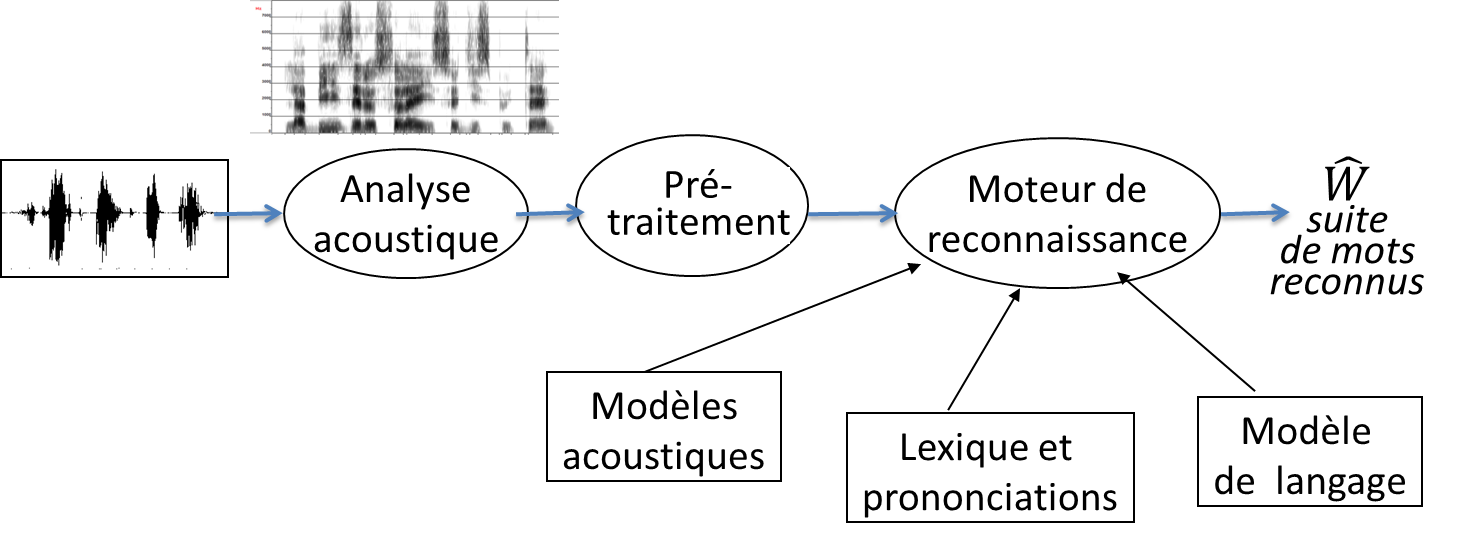
\includegraphics[scale=0.6]{img/schema_reco.png}}
  \caption{Schéma d'un système classique de reconnaissance de la parole}
\end{figure}

\noindent Ici, les éléments qui vont changer d'un langage à l'autre sont les modèles acoustiques, le lexique et les prononciations et le modèle de langage.\cite{jodouin90}\\
 \\
L'objectif de ce projet d'initiation à la recherche est donc de parvenir à détecter automatiquement la langue parlée dans un fichier audio. Cette détection automatique pourrait permettre de directement transcrire la parole prononcée dans le fichier, en utilisant la "bibliothèque" vocale correspondant à la langue parlée.\\
 \\
Pour ce faire, on utilisera des méthodes d'apprentissage automatique (machine learning) basées sur des réseaux de neurones profonds.
Dans un premier temps, le but sera de construire un réseau de neurones capable de déterminer, pour un fichier de parole homogène (même langue dans le fichier) donné en entrée, s'il s'agit de parole  allemande, anglaise, arabe ou française.\\
Ensuite, selon les performances du réseau précédent, nous tenterons de créer un système capable de détecter la langue d'un contenu audio de manière dynamique. Ainsi, nous pourrions repérer automatiquement, par exemple, une citation prononcée en anglais dans un flux de parole globalement allemande, pour pouvoir ainsi faciliter la transcription automatique d'un tel texte.

\section{Présentation générale}

\section{Prétraitement : préparation des données}

\section{Utilisation des réseaux de neurones}

\section{Conclusion}

\end{document}
